\documentclass{beamer}
\usepackage[utf8]{inputenc}
\usepackage[T1]{fontenc}

\usepackage{qtree}
\usepackage{dirtree}

\usebackgroundtemplate{
	
\includegraphics[width=\paperwidth,height=\paperheight]{img/background}
}

\title{Chapter 01: Structured Analysis}

\author[P.A. Nugroho]{Pascal Alfadian Nugroho}
\institute[IF-UNPAR]{Program Studi Informatika, \\Universitas Katolik Parahyangan}

\begin{document}
	\begin{frame}
		\titlepage
	\end{frame}

	\section{Introduction}
	\begin{frame}{Introduction}
		\begin{itemize}
			\item Structured Analysis may be rarely used today, as Object-Oriented approach is more suitable
			\item However, \cite[page xvi]{Schach:2006:OCS:1207045} said teachers still refer to this though not heavily discussed
			\item In Informatika UNPAR, we have decided to keep teaching this topic, to cater for final projects that focuses on algorithms or techniques rather than a full-blown app.
			\item In this example, we will see references to languages that is as old as my dad (Ada, COBOL, etc).
		\end{itemize}
	\end{frame}
	
	\section{Specification Document}
	\subsection{Overview}
	\begin{frame}{Specification Document}
		\begin{itemize}
			\item Contract between client and developer
			\item Specifies precisely what the product must do and constraints of the product
			\item Almost always, includes deadline
			\item Includes set of acceptance criteria
			\item \textbf{Does not} specify how the product is made unless specifically needed
			\item There can be many ways in writing a specification document
		\end{itemize}
	\end{frame}
	\subsection{Example}
	\begin{frame}{Specification Document: Example}
		\begin{center}
			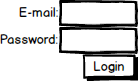
\includegraphics[scale=0.5]{img/01_login}
		\end{center}
		\begin{enumerate}
			\item The login screen must show two inputs: email and password
			\item Password must be transmitted securely to server using HTTPS
			\item The error message for ``unregistered user'' and ``invalid password`` must be exactly the same
			\item \textit{The login screen must be implemented using HTML5 and CSS3 standard} % example of requirement that specifically governs how the product is made
		\end{enumerate}
	\end{frame}
	\subsection{Goals}
	\begin{frame}{Specification Document: Goals}
		\begin{itemize}
			\item Agreement between client/user and development team
			\item Let development team fully understands the problem
			\item Hence a \textit{solution strategy}(-ies) can be suggested
		\end{itemize}
	\end{frame}

	\section{Informal Specifications}
	\subsection{Overview}
	\begin{frame}{Informal Specifications}
		Example of informal specification using \textit{natural language} \cite[page 462]{Schach:2006:OCS:1207045}:
		\begin{quotation}
		BV.4.2.5. If the sales for the current month are below the target sales, then a report is to be printed, unless the difference between target sales and actual sales is less than half of the difference between target sales and actual sales in the previous month or if the difference between target sales and actual sales for the current month is under 5 percent.
	\end{quotation}
	\end{frame}
	\subsection{Problems}
	\begin{frame}{Informal Specifications: Problems}
		\begin{itemize}
			\item Lengthy sentence to explain accurately what the product should behave
			\item Ambiguous, e.g. when comparing to last month, is it in terms of percentage or in dollars?
		\end{itemize}
	\end{frame}	

	\section{Structured Analysis}
	\subsection{Overview}
	\begin{frame}{Structured Analysis}
		\begin{columns}[t,totalwidth=\textwidth]
			\column{.5\linewidth}
				\begin{itemize}
					\item A more formal way of specification
					\item Use of graphics for specification was an important technique in 1970s (until today)
					\item Several techniques become popular, but we will use Gane and Sarsen \cite{gane1977structured} as suggested in main reference
					\item That is, a nine-step technique (summary on the right, explained in detail later)
				\end{itemize}
			\column{.5\linewidth}
			\begin{flushright}
				\small{
					\begin{enumerate}
						\item Draw the \textbf{Data Flow Diagram} (DFD) of existing system
						\item Decide what sections to computerize and how
						\item Determine the details of the data flows
						\item Define the logic of the process
						\item Define the data source
						\item Define the physical resources
						\item Determine the input-output specifications
						\item Perform the sizing
						\item Determine the hardware requirements
					\end{enumerate}
				}
			\end{flushright}
		\end{columns}		
	\end{frame}
	\subsection{Case Study: Sally's Software Show}
	\begin{frame}{Case Study: Sally's Software Show}
		\begin{itemize}
			\item Buys software from various suppliers and sells it to public
			\item Monthly turnover of 300 packages
			\item Average retail cost of \$250 each
			\item Analysis:
			\begin{itemize}
				\item Which parts should be computerized?
				\item What's the objective to computerize?
				\item Assumption: Sally wishes to computerize ``to make more money''
			\end{itemize}
		\end{itemize}
	\end{frame}
	\subsection{Step 1: Draw The DFD}
	\begin{frame}{Step 1: Draw The DFD}
	    \begin{small}
    		\begin{center}
    			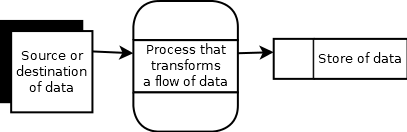
\includegraphics[scale=0.4]{img/01_dfd_symbols}
    		\end{center}	
    		\begin{itemize}
    			\item A pictorial representation of all aspects of the logical data flow
    			\item Constructed by identifying the \textbf{data flows}
    			\item Each flow of data starts and ends either at
    			\begin{itemize}
    				\item \textbf{Source or destination of data} (double-square box) or
    				\item \textbf{Data store} (open-ended rectangle)
    			\end{itemize}
    			\item Data are transformed by one or more \textbf{process}es (rounded rectangle)
    			\item Note diagrams in this presentation uses open source application ``Dia''.
    		\end{itemize}
		\end{small}
	\end{frame}
	\begin{frame}{Step 1: Draw The DFD}
		\begin{columns}[t,totalwidth=\textwidth]
			\column{.5\linewidth}
				\begin{itemize}
					\item DFD is generally large, therefore need to be developed in stepwise refinement
					\item On the right is example for Sally's Software Shop, first refinement
					\item That diagram can have many intepretations
					\item See two possible implementation (among others) in next slide
				\end{itemize}			
			\column{.5\linewidth}
				\begin{flushright}
					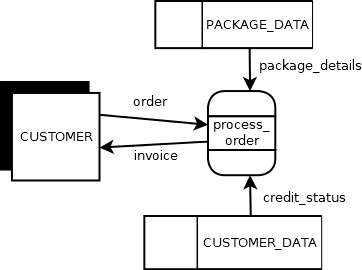
\includegraphics[scale=0.5]{img/01_sally_dfd_first_refinement}
				\end{flushright}
		\end{columns}
	\end{frame}
	\begin{frame}{Step 1: Draw The DFD}
		\begin{columns}[t,totalwidth=\textwidth]
			\column{.5\linewidth}
				Implementation 1: Manual
				\begin{itemize}
					\item PACKAGE\_DATA: physical CDs
					\item CUSTOMER\_DATA: small cards, like \textit{kartu berobat} (patient card)
					\item process\_order: taking note of the purchase in the card
				\end{itemize}
			\column{.5\linewidth}
				Implementation 2: Computerized
					\begin{itemize}
						\item PACKAGE\_DATA: computer file
						\item CUSTOMER\_DATA: computer file
						\item process\_order: entering input to the computerized system
					\end{itemize}
		\end{columns}
	\end{frame}
	\begin{frame}{Step 1: Draw The DFD}
		\begin{center}
			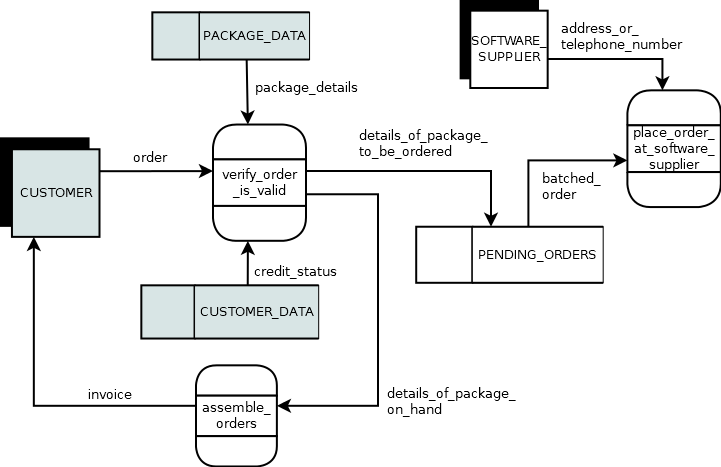
\includegraphics[scale=0.3]{img/01_sally_dfd_second_refinement}
		\end{center}	
		\begin{itemize}
			\item Second refinement of DFD, if an item requested is not available
			\item Notice that the DFD can't capture branching (\textit{if} statements)
		\end{itemize}
	\end{frame}
	\begin{frame}{Step 1: Draw The DFD}
		\begin{columns}[t,totalwidth=\textwidth]
			\column{.5\linewidth}
				\begin{itemize}
					\item Third refinement of DFD, focuses on financial functions
					\item DFD becomes large, and some other details omitted.
				\end{itemize}
			\column{.5\linewidth}
				\begin{flushright}
					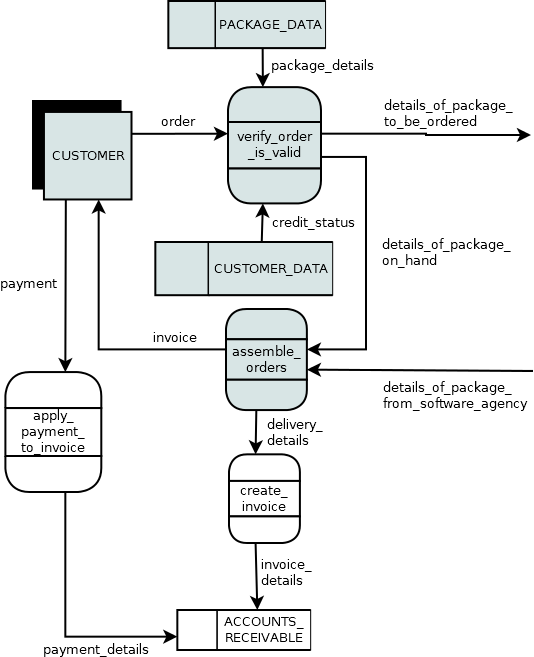
\includegraphics[scale=0.3]{img/01_sally_dfd_third_refinement}
				\end{flushright}
		\end{columns}
	\end{frame}
	\begin{frame}{Step 1: Draw The DFD}
		\begin{itemize}
			\item 1st, 2nd, etc... refinements sometimes known as DFD level 1, 2, etc... %locally known in IF-UNPAR%
			\item The more refinements, the larger the diagram. Hence can be divided hierarchically.
			\item A single box (process) at one level is expanded into a complete DFD at lower level.
		\end{itemize}
	\end{frame}

	\subsection{Step 2: Decide What Sections to Computerize and How}
	\begin{frame}{Step 2: Decide What Sections to Computerize and How}
		\begin{itemize}
			\item Ideally all operations are computerized, but cost may prohibit.
			\item For computerized operations, further question is whether to do it in batch or online
			\begin{itemize}
				\item Batch processes bulk of data (e.g. ``Upload CSV file'')
				\item Online process operation in time.
			\end{itemize}
		\end{itemize}
	\end{frame}

	\subsection{Step 3: Determine Details of Data Flows}
	\begin{frame}[fragile]{Step 3: Determine Details of Data Flows}
		\begin{itemize}
			\item Identify what data items must go into various data flows.
			\item Example:
\begin{verbatim}
order:
    order_identification
    customer_details
    package_details
\end{verbatim}
			\item In case of larger product, data dictionary keeps track of all data elements.
			\item Example of data dictionary in next slide.
		\end{itemize}
	\end{frame}
	\begin{frame}{Step 3: Determine Details of Data Flows}
		\begin{tiny}
			\begin{table}[]
			\caption{Example of data dictionary}
			\centering
			\begin{tabular}{| l | l | p{5cm} |}
			\hline
			\textbf{Name of Data Element} & \textbf{Description}                                                                                                                                                                                                         & \textbf{Narrative}                                                                                                                                                                                                                  \\ \hline
			order                         & \begin{tabular}[c]{@{}l@{}}Record comprising fields\\-order\_identification\\-customer\_details\\-customer\_name\\-customer\_address\\-...\\-package\_details\\-package\_names\\-package\_price\end{tabular} & The field contain all details of an order                                                                                                                                                                                           \\ \hline
			order\_identification         & 12 digit integer                                                                                                                                                                                                             & Unique number generated by procedure generateorder\_number. The first 10 digits contain the order number itself, the last 2 digits are check digits.                                                                                \\ \hline
			verify\_order\_is\_valid      & \begin{tabular}[c]{@{}l@{}}Procedure:\\-Input parameter:\\--order\\-Output parameter:\\--number\_of\_errors\end{tabular}                                                                                             & This procedure takes order as input and checks the validity of every fields; for each error found, an appropriate message is displayed on the screen (the total number of errors found is returned in parameter number\_of\_errors) \\ \hline
			\end{tabular}
			\end{table}
		\end{tiny}
	\end{frame}

	\subsection{Step 4: Define the Logic of the Process}
	\begin{frame}{Step 4: Define the Logic of the Process}
		\begin{itemize}
			\item For each process, investigate what happens within each process.
			\item For example, what would be the logic for \texttt{give\_educational\_discount}?
			\item We can use decision tree instead of natural language for more precision.
		\end{itemize}
		\Tree [.Discount [.{Educational institution} {<= 4 packages: 10\%} {> 4 packages: 15\%} ] {Other: 0\%} ]
	\end{frame}

	\subsection{Step 5: Define the Data Stores}
	\begin{frame}{Step 5: Define the Data Stores}
		\begin{itemize}
			\item Down to implementation, to define exact contents of each store and its representation.
			\item For COBOL, it means it has to be provided down to ``pic'' level. In Ada, ``digits'' or ``delta'' must be specified.
			\item (Fast forward today) For SQL, table structure can be used
		\end{itemize}
		\begin{table}[]
		\caption{Table ``products''}
		\centering
		\begin{tabular}{|l|l|l|}
		\hline
		\textbf{Name} & \textbf{Type} & \textbf{Extras}             \\ \hline
		id            & INT(11)       & Primary Key, Auto Increment \\ \hline
		name          & VARCHAR(256)  &                             \\ \hline
		price         & DECIMAL(20,2) &                             \\ \hline
		stock         & INT(11)       &                             \\ \hline
		\end{tabular}
		\end{table}
	\end{frame}

	\subsection{Step 6: Define the Physical Resources}
	\begin{frame}{Step 6: Define the Physical Resources}
		\begin{itemize}
			\item Also about implementation, determine representation of each element
			\item That is, the file organization and structure.
			\item \cite{Schach:2006:OCS:1207045} mentions about table structure similar to what I have explained in step 5. However, in our case let's stick to files only.
		\end{itemize}
		\dirtree{%
		.1 /. 
		.2 log/. 
		.3 \textit{YYYYMMDDHHIISS}.log. 
		.2 etc/. 
		.3 sally.conf. 
		}
	\end{frame}
	\begin{frame}{Step 6: Define the Physical Resources}
		\dirtree{%
		.1 /. 
		.2 log/. 
		.3 \textit{YYYYMMDDHHIISS}.log. 
		.2 etc/. 
		.3 sally.conf. 
		}
		\begin{small}
			\begin{quote}
			Log files (*.log) contains one log entry per line, where each line starts with \textit{YYYY-MM-DD HH:II:SS} followed by a tab, a log level (which can be either ``INFO'', ``NOTICE'', or ``ERROR''), another tab, an the log message. Each line is ended with a UNIX-style end-of-line.
			\end{quote}
			\begin{quote}
			The first line on \texttt{sally.conf} file is the number of lines followed. Each next line correspons to a key/value pair, separated with equal sign (``=''). Key must be in alphanumeric, while value can be all characters, ended with UNIX style end-of-line.
			\end{quote}
		\end{small}
	\end{frame}	

	\subsection{Step 7: Define the Input-Output Specifications}
	\begin{frame}{Step 7: Define the Input-Output Specifications}
		\begin{itemize}
			\item In this step, the input and output must be specified.
			\item If the app has graphical user interface, you could do a mockup. Better to use real input/output format instead of \textit{lorem ipsum}
			\item The app may take input from command line, console text input, or automatically from file. In that case, it has to be clearly defined instead of omitted.
			\item: Hint: try typing \texttt{java -help} in your console.
		\end{itemize}
	\end{frame}

	\subsection{Step 8: Define the Sizing}
	\begin{frame}{Step 8: Define the Sizing}
		\begin{itemize}
			\item It is necessary to predict the size of input (100 transactions per day? 1K? 1M?)
			\item This will be beneficial for the next step (hardware requirements)
		\end{itemize}
	\end{frame}

	\subsection{Step 9: Determine the Hardware Requirements}
	\begin{frame}{Step 9: Determine the Hardware Requirements}
		\begin{itemize}
			\item Determine the hardware requirement, e.g. memory, CPU, hard drives, etc...
			\item Useful to see if the app can run on current hardware, or to propose purchasing a new one.
		\end{itemize}
	\end{frame}

	\subsection{Conclusion}
	\begin{frame}{Conclusion}
		\begin{itemize}
			\item This (Gane and Sarsen) technique does not provide the answer to every question.
			\item For example: response times, timing, etc...
			\item However, at its time, it led to major improvements in the ways products were specified.
			\item Takeaway: you can use both the \textbf{9-step technique} and \textbf{Data Flow Diagram} to specify your app in your final project.
		\end{itemize}
	\end{frame}

	\section{References}
	\begin{frame}[allowframebreaks]
	        \frametitle{References}
	        \bibliographystyle{amsalpha}
	        \bibliography{module_01}
	\end{frame}
\end{document}

